\section{Backhual Network Channel Assignment}
\label{sec:whitemesh}

% Organization of the Sec
In this section, we formulate the channel assignment problem use WiFi and white space bands in concert 
when deploying wireless backhual networks. We then present our integer linear programming model and 
heuristic algorithm to address the problem. 
 
\subsection{WhiteMesh Backhual Architecture}
\label{subsec:architecture}

% Explain multiband vs multichannel Adding channel occupancy here, and also activity level
Many works which rely on such an assumption have focused on the allocation of multiple WiFi channels 
with multiple radios in multihop wireless networks with channels in one band~\cite{doraghinejad2014channel}.
However, as white space bands come to this problem, the propagation variation has to be considered in 
wireless network deployment. The propagation variation brings both spatial and spectrum variation for 
backhual network design.

In this work, we consider the diverse propagation characteristics for four frequency bands: 450 MHz, 800 
MHz, 2.4 GHz, and 5.8 GHz. We refer to the two former frequency bands as white space (WS) bands, whereas
the two latter frequency bands as WiFi bands. Due to the broadcast nature of the wireless medium, 
greater levels of propagation induce higher levels of interference. Also, the more allowed frequency
channels and low level signal activity of white space bands co-exist in sparse areas. Thus, in 
sparsely-populated rural areas, the lower frequencies of the white space bands might be a more appropriate 
choice for multihop paths to gateways having reduced hop count with more capacity. However, as the population 
and demand scales up (e.g., for urban regions), the reduced spatial reuse and greater levels of interference 
of white space bands might detract from the overall channel assignment strategy. In such urban areas, select 
links of greater distance might be the most appropriate choice for white space bands, especially since the 
number of available channels is often inversely proportional to the population (due to the existence of greater 
TV channels).

\subsection{Model and Problem Formulation}
\label{subsec:problem}

To distinguish the dynamics of white space bands, we employ the activity level based on multiple measurements 
in the target area to represent the achieved channel capacity. Correspondingly, a connectivity graph $C$ is 
formed for each band in $B$ such that $C=(V,L,B)$.  If the received signal for a given band is above an 
interference-range threshold, then contention occurs between nodes. 

We extend the conflict matrix in~\cite{tang2005interference} related to various interference per band according 
to $F=(E_{i,j},I_{Set},B)$, where $E_{i,j}$ represents the link and $I_{Set}$ includes all the links are physically 
inside the interference range $D_r$ when operating on each band $b \in B$.

Therefore, the problem we model is: to choose the connectivity graph $C'$ which maximizes the served traffic flow obey 
the constraints of multiband wireless network (defined below). A key challenge is that selecting the optimal channels from
the set $B$ leads to a conflict graph $F$ which cannot be known {\it a priory}. Previous works have proposed several 
coloring, cluster-independent set, mixed linear integer methodology for a single band $b$
~\cite{peng2012efficient,tang2005interference,doraghinejad2014channel}. 
However, these works do not address a reduction in hop count or an increase in spatial reuse and channel occupancy for 
a set of diverse bands $B$. 

% Metrics
In network application, the bottleneck of mesh network capacity has been shown to be the gateway's wireless 
connections~\cite{robinson2008adding}. The metric we use to evaluate the proposed algorithm is the served traffic flow.
Wireless networks are operated and maintained by vendors, such as AT\&T, T-Mobile, who charge the customers based on their data 
through Internet. In practice, the traffic demand of the user obey Poisson distribution\cite{saaty1961elements}, 
we then generated Poisson distributed numbers to represent clients' traffic demands in our simulation. The served traffic 
flow is correlated to the population of the area since each user has similar traffic demand in long term average. The 
employed performance metric of served traffic flow $X$, is represented the traffic arrived at the gateway nodes, where 
in Eq.~\ref{eq:goodput}:
\begin{equation}
\label{eq:goodput}
X=\sum_{w \in W, v \in V}T(w,v)
\end{equation}
The traffic arrived gateway node $w\in W$ considers all incoming and outgoing wireless traffic from access node $v\in V$ 
as $T$ onto the Internet. Obviously, the served traffic flow is also related to the routing and other factors, we use a 
simple routing method to keep the maximum the traffic arrived at the gateway nodes, the exact calculation of served traffic
flow is described in Section~\ref{subsec:wmanalysis}.

\subsection{Linear Programming Formulation}
\label{subsec:linearopt}

To clarify the problem and approach the optimization solution of the problem, we present a linear programming 
formulation for optimizing channel assignment in multiband scenario. We assume that the set of available mesh nodes 
($V$), gateways ($W$), and available bands ($B$) are pre-known. The communication links and conflict graph are 
given as parameters. The capacity $\delta_b$ is given as the achieved channel capacity from the  activity level 
measurement calculation in~\ref{eq:intercap}. 


% Start from here on Fri, finish in the morning
\noindent
{\bf Sets:}
\begin{tabular}{ll}
$V$ & set of nodes \\
$B$ & set of bands \\
\end{tabular}

\noindent
{\bf Parameters:}\\
\\
%\vspace{0.1in}
%\begin{tabular}{lll}
\begin{tabular}{llp{3.4cm}}
%\hline
$\delta^b$ & $b \in B$ & Available capacity of band $b$ in target area\\
%\begin{tabular}{llp{2.8cm}}
$I_{ij,lm}^b$ & $(i,j,l,m) \in V, b\in B $ & Protocol Interference of link $(i,j)$ on band $b$ brought by link $(l,m)$\\
%\hline
%\end{tabular}\\
%\begin{tabular}{llp{2.8cm}}
$W_i$ & $i \in V\ binary$ & Gateway maker in mesh nodes\\
%\hline
%\end{tabular}\\
%\begin{tabular}{llp{2.8cm}}
$D_{d}$ & $i \in V\ $ & Downlink demand of node i\\
%\hline
%\end{tabular}\\
%\begin{tabular}{llp{2.8cm}}
$D_{u}$ & $i \in V\ $ & Uplink demand of node i\\
%\hline
\end{tabular}

In the variable set, we define a time share represents the percentage of time a single link transmits according 
to~$\alpha_{i,j}^b$ for link $i,j$ between node $i$ and node $j$ in band $b$. There are two terms $uy_{i,j,k}^{b}$
and $dy_{i,j,k}^{b}$ defined as uplink and downlink flows:

\noindent
%\vspace{2pt}
{\bf Variables:}\\
\\
%\vspace{1pt}
\begin{tabular}{llp{3cm}}
$0\le \alpha_{ij}^b \le 1$  & $b\in B, (i,j) \in N$ & 
Time share of link $(i,j)$ on band $b$\\ 
$0\le uy_{i,j,k}^b$ & $(i,j,k) \in V, b \in B$ & 
Uplink flow of node $k$ on link $(i,j)$ at band $b$ \\ 
$0\le dy_{i,j,k}^b$ & $(i,j,k) \in N, b \in B$ & 
Downlink flow of node $k$ on link $(i,j)$ at band $b$ \\ 
\end{tabular}
\vspace{1pt}

% FIXME talk about NT calculation
Our objective is represented for  
maximizing the traffic arrived at gateway ($X$)
described in Eq.~\ref{eq:goodput}.

\noindent
{\bf Objective:}
\begin{align}
& Max \sum_i\sum_j\sum_k\sum_b(uy_{i,j,k}^b+dy_{j,i,k}^b) \;\ When \; w_j=1 
%& Max \sum_i\sum_j\sum_b(\frac{1}{\sum_{l,m}\alpha_{i,j}^b\times I_{ij,lm}})
\end{align}

In the ILP, the connectivity, uplink, and downlink constraints are represented as:  

\noindent
%{\bf Constraints:}
{\bf Connectivity Constraints:}
\begin{align}
\label{opt:1}
& \alpha_{i,j}^b + \alpha_{j,i}^b + \sum_l\sum_m(\alpha_{l,m}^b \cdot I_{ij,lm}^b) \leq \delta^b, i\neq j \\
\label{opt:2}
& \sum_i uy_{i,j,k}^b + \sum_i dy_{i,j,k}^b \leq \delta^b \cdot \alpha_{j,k}^b 
\end{align}
\noindent
{\bf Uplink Constraints:} 
\begin{align}
\label{opt:3}
& \sum_k \sum_b uy_{i,k,i}^b \leq D_{ui}  \; ; w_k=0, i \neq k \\
\label{opt:4}
& uy_{i,j,k}^b \cdot w_k = 0 \\
%\label{opt:5}
%& \sum_i\sum_b uy_{i,j,k}^b - \sum_m\sum_b uy_{j,m,k}^b = 0 \; when \; w_k=0, i\neq k\\
\label{opt:6}
& \sum_{i\leq j}\sum_b uy_{i,j,k}^b = \sum_{m\leq j} \sum_b uy_{j,m,k}^b \; ;w_j = 0\\
\label{opt:7}
& uy_{i,j,i}^b=0 
\end{align}
\noindent
{\bf Downlink Constraints:} 
\begin{align}
{\bf}
\label{opt:8}
& \sum_k \sum_b dy_{i,k,i}^b \leq D_{di} \; \; ; w_k=0 \\
\label{opt:9}
& dy_{i,j,k}^b =0  \; ;w_k=1 \\
%\label{opt:10}
%& \sum_j\sum_b dy_{i,j,k}^b - \sum_m\sum_b dy_{i,k,m}^b \geq , i \neq k \\
\label{opt:11}
& \sum_{i\neq j} \sum_b dy_{i,j,k}^b = \sum_{m \neq j} \sum_b dy_{j,m,k}^b   \; ; w_j=0, i \neq k \\
\label{opt:12}
& dy_{i,i,j}^b=0
\end{align}

In the constraints, (\ref{opt:1}) represents the summation of the incoming and outgoing wireless time 
share and the interfering links' wireless time share, which should all be less than 1. Constraint (\ref{opt:2}) 
represents the incoming and outgoing wireless traffic, which should be less than the link capacity for 
link $i,j$. Uplink constraints (\ref{opt:3}) and (\ref{opt:4}) represent that the summation of any wireless 
flow $i,j$ should be less than the demand of node $k$.  Constraints (\ref{opt:6}) and (\ref{opt:7}) are used 
to restrict the sum of all incoming data flows for a given mesh node $k$ to be equal to the sum of all outgoing 
flows. Downlink constraints (\ref{opt:8}) and (\ref{opt:9}) are similar to (\ref{opt:3}) and (\ref{opt:4}) but 
in the downlink direction.  Similarly, constraints (\ref{opt:11}) and (\ref{opt:12}) are downlink versions of 
(\ref{opt:6}) and (\ref{opt:7}).

Similar linear programs model is to solve channel assignment wireless networks have been proved to be NP-hard
~\cite{yuan2006cross}. Our model jointly considers channel assignment factors and multiband scenario which is more
complex . When the particular configuration is given, we further choose the objectives, parameters, and relax 
constraints to find the approaching solution for the network.  

%\section{Path Analysis with Diverse Propagation}
\label{sec:wmalgorithms}


In this section, we discuss the influence of diverse propagation
characteristics of the wide range of carrier frequencies of
% NEWClaim fix
white space and WiFi bands. We then introduce our measurement 
driven heuristic algorithm for channel assignment in 
WhiteMesh networks.

% PEN part 
\subsection{Path Interference Induced on the Network}
\label{subsec:PEN}

In WhiteMesh networks, multihop paths can be intermixed with WiFi 
for more spacial reuse and white space bands with less hops.  
To deal with the trade-off, we consider
analyze the band choices reduce the number of hops along a path and the 
aggregate level of interference that hop-by-hop path choices have
on the network (i.e., Path Interference induced on the Network).

Mesh nodes closer to the gateway generally achieve
greater levels of throughput at sufficiently high offered loads. 
To combat such starvation effects, we treat each flow with equal priority in the network when
assigning channels. In the worst case, all nodes along a particular path have equal 
time shares for contending links (i.e., intra-path interference).
We start the channel assignment assuming that $h$ mesh nodes are demanding
traffic from each hop of an $h$-hop path to the gateway. If each link along the 
path uses orthogonal channels, then each link could be active simultaneously,
otherwise they will complete with each other. 
We note each node along the path had traffic demand $T_d$, obviously the bottleneck 
link along the path would be the one closest to the gateway, and then next. 
Thus, the total traffic along the path $h \cdot T_d$ must be less than the 
bottleneck link's capacity $\delta$ estimated from the measurements. In such a scenario, the $h$-hop mesh node 
would achieve the minimum served demand, which we define as the network efficiency. 
In general, the active time per link for an $h$-hop mesh node can be represented 
by $1,\frac{h-1}{h},\frac{h-2}{h}\cdots \frac{1}{h}$. The summation of all active 
times for each mesh node along the path is considered the intra-path network cost.

Considering only intra-path interference, using lower carrier frequencies allows a
reduction in hop count and increase in the network efficiency of each mesh node along
the $h$-hop path. However, a lower carrier frequency will induce greater interference
to other paths to the gateway (i.e., inter-path interference). 
Fig.~\ref{fig:interferencerange} depicts such an example where
links in different bands are represented by circles for 450 MHz, rectangles for
2.4 GHz, and triangles for the nodes which can choose between the two.
Nodes $A$ and $C$ could be connected through two 2.4-GHz links or a single 450-MHz link.
With 2.4 GHz, the interfering distance will be less than using 450 MHz. For example, only 
link $D,E$ will suffer from interference, whereas $H,I$ would not. However, with 450 MHz,
link $A,C$ would interfere with links $F,G$, $M,L$, and $K,J$. At each time unit, the number of
links interfering with the active links along a path would be the inter-path network cost.

When an $h$-hop flow is transmitted to a destination node, it prevents 
activity on a number of links in the same frequency via the protocol model. 
The active time on a single link can be noted as 
$\frac{T}{\gamma_h}$. 
An interfering link from the conflict matrix $F$ counts as $I_h$ per unit time
and contributes to the network cost in terms of:
$\frac{hT}{\gamma_1}\cdot I_1 + \frac{(h-1)T}{\gamma_2}\cdot I_2 \cdots \frac{T}{\gamma_h}\cdot I_h$.
Then, the traffic transmitted in a unit of network cost for the $h$-hop node is:
\begin{equation}
\label{eq:originpen}
E_{\eta}=\frac{T}{\sum_{i \in h}\frac{(h-i+1)\cdot T}{\gamma_i}\cdot I_i }
\end{equation}
Using network efficiency, the equation simplifies to:
\begin{equation}
\label{eq:pen}
E_{\eta}=\frac{\gamma}{\sum_{i \in h} (h-i+1)\cdot I_i}
\end{equation}

The network efficiency is the amount of traffic that could be 
offered on a path per unit time. With multiple channels from the same band,
$I_i$ will not change due to the common communication range. With multiple
bands, $I_i$ depends on the band choice due to the communication range diversity.  
This network efficiency jointly considers hop count and interference. We define
the Path Interference induced on the Network (PIN) as the denominator of Eq.~\ref{eq:pen},
which represents the sum of all interfering links in the network by a given path. 
PIN is used to quantify the current state of channel for channel assignment
across WiFi and white space bands.
To determine when the lower carrier frequency will be better than two or more hops at a
higher carrier frequency, we consider the average interference $\bar{I}$ of a given path
at the higher frequency.  The problem could be formulated as:
\begin{equation}
\label{eq:benefit}
\frac{\gamma}{\frac{h(h-1)}{2}\cdot \bar{I}+I_x} \geq \frac{\gamma}{\frac{h(h+1)}{2}\cdot \bar{I}}
\end{equation}

Here, from Eq.~ref{eq:benefit} when $I_x \leq 2\cdot h\bar{I}$, the performance of a lower-frequency link  
is better than two higher-frequency hops for the same destination node. $I_x$ is also a parameter of hop count 
in Eq.~\ref{eq:pen}. When the hop count is lower which closer to the gateway node, the threshold 
would be more strict since the interference would have a greater effect on the performance.




\subsection{Band-based Path Selection (BPS) Algorithm}
\label{subsec:BPS}

\begin{algorithm}[t]
    \small
\caption{Band-based Path Selection (BPS)}
\label{algorithms:bps}
\begin{algorithmic}[1]
\REQUIRE  ~~\\
	$M$: Set of mesh nodes\\
	$G$: Set of gateway nodes\\
	$C$: Communication graph of potential links among all nodes\\
	$I$: Interference matrix of all potential links \\
	$B$: Available frequency bands \\
	$\delta$: Measurements based Channel Capacity
\ENSURE ~~\\    
$CA$: Channel Assignment of the Network\\
\STATE Rank mesh nodes in Set $M$ according to physical distance from gateway nodes $G$
\STATE Initialize $S_{curr}=G$, $N_{srv}=\emptyset$, $N_{unsrv}=M$,$I_{active}=\emptyset$
\WHILE {$N_{srv}=!M$}
\STATE Select node with largest distance to gateway
\STATE Find the adjacency matrix across band combinations $A_c$
\FORALL{$A_{i}\in A_c$}
\STATE Find the shortest path $SP_i$ in mixed adjacency matrix A 
\FORALL{Link $l \in SP_i$, ordered from gateway to mesh node}
\STATE Find the least interfering path with measured $\delta \times E_n$
\STATE If equally-interfering links, choose higher frequency
\STATE Calculate the path interference of $SP_i$
\ENDFOR
\STATE Store the shortest path $SP_i$ as $SP$
\ENDFOR
\STATE Assign the path in the network\\
		\STATE Update $N_{srv},N_{unsrv}$
		\STATE Update $I_{active}$ from $I$
\ENDWHILE 

Output $CA$ as the locally-optimal solution\\
\end{algorithmic}
\end{algorithm}

We design a Band-based Path Selection (BPS) algorithm
(described in Alg.~\ref{algorithms:bps}) which first chooses the 
mesh node that has the largest physical distance from the gateway 
nodes to reduce the whole time cost of the network. When a path is constructed for
the mesh node with the greatest distance, all subsequent mesh nodes along
the path are also connected to the gateway. The intuition behind the
BPS algorithm is to improve the worst mesh node performance in a path.
In large-scale mesh networks, it is impractical to traverse all the paths with
different combination of bands from a mesh node to any gateway node since 
it is a NP-hard problem. However,
based on the discussion in Section~\ref{subsec:PEN}, if two paths have the same
number of used bands along those paths, then the path with the least hops
is likely to have the greatest performance and is chosen.  Similarly, if
two path have the same path interference, we choose the path which has
higher-frequency links for spatial reuse. Thus, the next step of the
algorithm is to find the shortest path across band combinations.

To run the algorithm, compared to the number of mesh nodes, the amount of channels $N_B$ in
different bands is small. The time complexity of calculating the combination
is $O(2^{N_B})$. Finding the shortest path in Dijkstra algorithm will
cost $O(N_E^2)$ according to~\cite{golden1976shortest}, where $N_E$ is the set of possible links in the
network, and as a result, the total complexity would be $O(N_E^2\cdot 2^{N_B})$.
The algorithm would then calculate the PIN of the candidate path and select the path
with the least interference channel induced on the network for the source mesh node.
After a path is assigned, the algorithm updates the network's channel assignment
with served nodes, activated links, and radio information. Then,
we iteratively assign channels for all the mesh nodes in the
network.

If all the nodes are connected to gateway nodes ($N_E={n \choose 2}$ which is $O(N_V^2)$), 
then the complexity of assigning a channel for a mesh node is $O(N_E^2\cdot2^{N_B})$. 
Then, the complexity of assigning a mesh node is $O(N_V^4\cdot2^{N_B})$.
To assign {\it all} the nodes in the network, the complexity would 
be $O(N_V^5\cdot2^{N_B})$. The complexity is polynomial time of
the number of traffic demands points (client group) for a wireless
network assignment.



\subsection{Path Analysis with Diverse Propagation}
\label{subsec:wmalgorithms}


We discuss the influence of diverse propagation characteristics of the wide range of carrier frequencies of
white space and WiFi bands in wireless networks. We then introduce our measurement driven heuristic algorithm 
for channel assignment in WhiteMesh networks.

% PEN part 
%\subsection{Path Interference Induced on the Network}
\label{subsec:PEN}

In WhiteMesh networks, multihop paths can be intermixed with WiFi 
for more spacial reuse and white space bands with less hops.  
To deal with the trade-off, we consider
analyze the band choices reduce the number of hops along a path and the 
aggregate level of interference that hop-by-hop path choices have
on the network (i.e., Path Interference induced on the Network).

Mesh nodes closer to the gateway generally achieve
greater levels of throughput at sufficiently high offered loads. 
To combat such starvation effects, we treat each flow with equal priority in the network when
assigning channels. In the worst case, all nodes along a particular path have equal 
time shares for contending links (i.e., intra-path interference).
We start the channel assignment assuming that $h$ mesh nodes are demanding
traffic from each hop of an $h$-hop path to the gateway. If each link along the 
path uses orthogonal channels, then each link could be active simultaneously,
otherwise they will complete with each other. 
We note each node along the path had traffic demand $T_d$, obviously the bottleneck 
link along the path would be the one closest to the gateway, and then next. 
Thus, the total traffic along the path $h \cdot T_d$ must be less than the 
bottleneck link's capacity $\delta$ estimated from the measurements. In such a scenario, the $h$-hop mesh node 
would achieve the minimum served demand, which we define as the network efficiency. 
In general, the active time per link for an $h$-hop mesh node can be represented 
by $1,\frac{h-1}{h},\frac{h-2}{h}\cdots \frac{1}{h}$. The summation of all active 
times for each mesh node along the path is considered the intra-path network cost.

Considering only intra-path interference, using lower carrier frequencies allows a
reduction in hop count and increase in the network efficiency of each mesh node along
the $h$-hop path. However, a lower carrier frequency will induce greater interference
to other paths to the gateway (i.e., inter-path interference). 
Fig.~\ref{fig:interferencerange} depicts such an example where
links in different bands are represented by circles for 450 MHz, rectangles for
2.4 GHz, and triangles for the nodes which can choose between the two.
Nodes $A$ and $C$ could be connected through two 2.4-GHz links or a single 450-MHz link.
With 2.4 GHz, the interfering distance will be less than using 450 MHz. For example, only 
link $D,E$ will suffer from interference, whereas $H,I$ would not. However, with 450 MHz,
link $A,C$ would interfere with links $F,G$, $M,L$, and $K,J$. At each time unit, the number of
links interfering with the active links along a path would be the inter-path network cost.

When an $h$-hop flow is transmitted to a destination node, it prevents 
activity on a number of links in the same frequency via the protocol model. 
The active time on a single link can be noted as 
$\frac{T}{\gamma_h}$. 
An interfering link from the conflict matrix $F$ counts as $I_h$ per unit time
and contributes to the network cost in terms of:
$\frac{hT}{\gamma_1}\cdot I_1 + \frac{(h-1)T}{\gamma_2}\cdot I_2 \cdots \frac{T}{\gamma_h}\cdot I_h$.
Then, the traffic transmitted in a unit of network cost for the $h$-hop node is:
\begin{equation}
\label{eq:originpen}
E_{\eta}=\frac{T}{\sum_{i \in h}\frac{(h-i+1)\cdot T}{\gamma_i}\cdot I_i }
\end{equation}
Using network efficiency, the equation simplifies to:
\begin{equation}
\label{eq:pen}
E_{\eta}=\frac{\gamma}{\sum_{i \in h} (h-i+1)\cdot I_i}
\end{equation}

The network efficiency is the amount of traffic that could be 
offered on a path per unit time. With multiple channels from the same band,
$I_i$ will not change due to the common communication range. With multiple
bands, $I_i$ depends on the band choice due to the communication range diversity.  
This network efficiency jointly considers hop count and interference. We define
the Path Interference induced on the Network (PIN) as the denominator of Eq.~\ref{eq:pen},
which represents the sum of all interfering links in the network by a given path. 
PIN is used to quantify the current state of channel for channel assignment
across WiFi and white space bands.
To determine when the lower carrier frequency will be better than two or more hops at a
higher carrier frequency, we consider the average interference $\bar{I}$ of a given path
at the higher frequency.  The problem could be formulated as:
\begin{equation}
\label{eq:benefit}
\frac{\gamma}{\frac{h(h-1)}{2}\cdot \bar{I}+I_x} \geq \frac{\gamma}{\frac{h(h+1)}{2}\cdot \bar{I}}
\end{equation}

Here, from Eq.~ref{eq:benefit} when $I_x \leq 2\cdot h\bar{I}$, the performance of a lower-frequency link  
is better than two higher-frequency hops for the same destination node. $I_x$ is also a parameter of hop count 
in Eq.~\ref{eq:pen}. When the hop count is lower which closer to the gateway node, the threshold 
would be more strict since the interference would have a greater effect on the performance.



\subsection{Path Interference Induced on the Network}
\label{subsec:PEN}

In WhiteMesh networks, multihop paths can be intermixed with WiFi for more spacial reuse and white space bands 
with less hops. To deal with the trade-off, we consider analyze the band choices reduce the number of hops along 
a path and the aggregate level of interference that hop-by-hop path choices have on the network (i.e., Path 
Interference induced on the Network).

Mesh nodes closer to the gateway generally achieve greater levels of throughput at sufficiently high offered loads. 
To combat such starvation effects, we treat each flow with equal priority in the network when assigning channels. 
In the worst case, all nodes along a particular path have equal time shares for contending links (i.e., intra-path 
interference). We start the channel assignment assuming that $h$ mesh nodes are demanding traffic from each hop of 
an $h$-hop path to the gateway. If each link along the path uses orthogonal channels, then each link could be active 
simultaneously, otherwise they will complete with each other. We note each node along the path had traffic demand 
$T_d$, obviously the bottleneck link along the path would be the one closest to the gateway, and then next. 
Thus, the total traffic along the path $h \cdot T_d$ must be less than the bottleneck link's capacity $\delta$ 
estimated from the measurements. In such a scenario, the $h$-hop mesh node would achieve the minimum served demand, 
which we define as the network efficiency. In general, the active time per link for an $h$-hop mesh node can be represented 
by $1,\frac{h-1}{h},\frac{h-2}{h}\cdots \frac{1}{h}$. The summation of all active times for each mesh node along the 
path is considered the intra-path network cost.

Considering only intra-path interference, using lower carrier frequencies allows a reduction in hop count and increase 
in the network efficiency of each mesh node along the $h$-hop path. However, a lower carrier frequency will induce 
greater interference to other paths to the gateway (i.e., inter-path interference). 
When an $h$-hop flow is transmitted to a destination node, it prevents 
activity on a number of links in the same frequency via the protocol model. 
The active time on a single link can be noted as 
$\frac{T}{\gamma_h}$. 
An interfering link from the conflict matrix $F$ counts as $I_h$ per unit time
and contributes to the network cost in terms of:
$\frac{hT}{\gamma_1}\cdot I_1 + \frac{(h-1)T}{\gamma_2}\cdot I_2 \cdots \frac{T}{\gamma_h}\cdot I_h$.
Then, the traffic transmitted in a unit of network cost for the $h$-hop node is:
\begin{equation}
\label{eq:originpen}
E_{\eta}=\frac{T}{\sum_{i \in h}\frac{(h-i+1)\cdot T}{\gamma_i}\cdot I_i }
\end{equation}
Using network efficiency, the equation simplifies to:
\begin{equation}
\label{eq:pen}
E_{\eta}=\frac{\gamma}{\sum_{i \in h} (h-i+1)\cdot I_i}
\end{equation}

The network efficiency is the amount of traffic that could be 
offered on a path per unit time. With multiple channels from the same band,
$I_i$ will not change due to the common communication range. With multiple
bands, $I_i$ depends on the band choice due to the communication range diversity.  
This network efficiency jointly considers hop count and interference. We define
the Path Interference induced on the Network (PIN) as the denominator of Eq.~\ref{eq:pen},
which represents the sum of all interfering links in the network by a given path. 
PIN is used to quantify the current state of channel for channel assignment
across WiFi and white space bands.
To determine when the lower carrier frequency will be better than two or more hops at a
higher carrier frequency, we consider the average interference $\bar{I}$ of a given path
at the higher frequency.  The problem could be formulated as:
\begin{equation}
\label{eq:benefit}
\frac{\gamma}{\frac{h(h-1)}{2}\cdot \bar{I}+I_x} \geq \frac{\gamma}{\frac{h(h+1)}{2}\cdot \bar{I}}
\end{equation}

Here, from Eq.~ref{eq:benefit} when $I_x \leq 2\cdot h\bar{I}$, the performance of a lower-frequency link  
is better than two higher-frequency hops for the same destination node. $I_x$ is also a parameter of hop count 
in Eq.~\ref{eq:pen}. When the hop count is lower which closer to the gateway node, the threshold 
would be more strict since the interference would have a greater effect on the performance.






\subsection{Band-based Path Selection (BPS) Algorithm}
\label{subsec:BPS}

\begin{algorithm}[t]
    \small
\caption{Band-based Path Selection (BPS)}
\label{algorithms:bps}
\begin{algorithmic}[1]
\REQUIRE  ~~\\
	$M$: Set of mesh nodes\\
	$G$: Set of gateway nodes\\
	$C$: Communication graph of potential links among all nodes\\
	$I$: Interference matrix of all potential links \\
	$B$: Available frequency bands \\
	$\delta$: Measurements based Channel Capacity
\ENSURE ~~\\    
$CA$: Channel Assignment of the Network\\
\STATE Rank mesh nodes in Set $M$ according to physical distance from gateway nodes $G$
\STATE Initialize $S_{curr}=G$, $N_{srv}=\emptyset$, $N_{unsrv}=M$,$I_{active}=\emptyset$
\WHILE {$N_{srv}=!M$}
\STATE Select node with largest distance to gateway
\STATE Find the adjacency matrix across band combinations $A_c$
\FORALL{$A_{i}\in A_c$}
\STATE Find the shortest path $SP_i$ in mixed adjacency matrix A 
\FORALL{Link $l \in SP_i$, ordered from gateway to mesh node}
\STATE Find the least interfering path with measured $\delta \times E_n$
\STATE If equally-interfering links, choose higher frequency
\STATE Calculate the path interference of $SP_i$
\ENDFOR
\STATE Store the shortest path $SP_i$ as $SP$
\ENDFOR
\STATE Assign the path in the network\\
		\STATE Update $N_{srv},N_{unsrv}$
		\STATE Update $I_{active}$ from $I$
\ENDWHILE 

Output $CA$ as the locally-optimal solution\\
\end{algorithmic}
\end{algorithm}

We design a Band-based Path Selection (BPS) algorithm (described in Alg.~\ref{algorithms:bps}) which 
first chooses the mesh node that has the largest physical distance from the gateway nodes to 
reduce the whole time cost of the network. When a path is constructed for the mesh node with 
the greatest distance, all subsequent mesh nodes along the path are also connected to the gateway. 
The intuition behind the BPS algorithm is to improve the worst mesh node performance in a path.
In large-scale mesh networks, it is impractical to traverse all the paths with different combination 
of bands from a mesh node to any gateway node since it is a NP-hard problem. However, based on the 
discussion in Section~\ref{subsec:PEN}, if two paths have the same number of used bands along those 
paths, then the path with the least hops is likely to have the greatest performance and is chosen. 
Similarly, if two path have the same path interference, we choose the path which has higher-frequency 
links for spatial reuse. Thus, the next step of the algorithm is to find the shortest path across 
band combinations.

To run the algorithm, compared to the number of mesh nodes, the amount of channels $N_B$ in
different bands is small. The time complexity of calculating the combination
is $O(2^{N_B})$. Finding the shortest path in Dijkstra algorithm will
cost $O(N_E^2)$ according to~\cite{golden1976shortest}, where $N_E$ is the set of possible links in the
network, and as a result, the total complexity would be $O(N_E^2\cdot 2^{N_B})$.
The algorithm would then calculate the PIN of the candidate path and select the path
with the least interference channel induced on the network for the source mesh node.
After a path is assigned, the algorithm updates the network's channel assignment
with served nodes, activated links, and radio information. Then,
we iteratively assign channels for all the mesh nodes in the
network.

If all the nodes are connected to gateway nodes ($N_E={n \choose 2}$ which is $O(N_V^2)$), 
then the complexity of assigning a channel for a mesh node is $O(N_E^2\cdot2^{N_B})$. 
Then, the complexity of assigning a mesh node is $O(N_V^4\cdot2^{N_B})$.
To assign {\it all} the nodes in the network, the complexity would 
be $O(N_V^5\cdot2^{N_B})$. The complexity is polynomial time of
the number of traffic demands points (client group) for a wireless
network assignment.


\subsection{Evaluation of WhiteMesh Backhual Channel Assignment}
\label{subsec:whitemeshexperimentdesign}

% Adjust the order of the results and explain the result more in detail
We now extensively evaluate our proposed measurement-driven heuristic algorithm against the 
upper bound approaching formed by our integer linear program and versus prior channel assignment 
strategies. We introduce the topologies and metric calculation used in the analysis and present a 
set of results based on the linear program and heuristic algorithm.

\subsection{Experimental Evaluation Setup}
\label{subsec:design}
% Simulation Setup
A key aspect of WhiteMesh networks is the diversity in propagation from the lowest white
space channels (tens to hundreds of MHz) to the highest WiFi channels (multiple GHz). Thus, 
to evaluate the performance of our measurement-driven algorithm, we consider a wide range 
of propagation characteristics from four different frequency bands.  
We have 450 MHz and 800 MHz in white space bands and 2.4 GHz and 5.8 GHz in WiFi bands
in previous measurement work.

% Network Setup
The measurements connect the relation of population distribution, traffic demand,
and available channel capacity in multiple bands. We input the measurements to the ILP and heuristic 
algorithm to calculate the available channel capacity $\delta$ for our algorithm which makes the available 
channel capacity of all the bands more practical. With the same transmission power and antenna gain, the 
highest carrier frequency would have the shortest communication range. Hence, we set a communication-range 
threshold of -100 dBm, and normalize the communication range with the highest frequency of 5.8 GHz. In 
particular, the communication range of 450 MHz, 800 MHz, 2.4 GHz, and 5.8 GHz would be normalized to 12.8, 
6.2, 2.4, and 1, respectively according to Eq.~\ref{eq:friis}. The interference range is computed as twice 
that of the communication range~\cite{raniwala2005architecture}. We deploy static wireless mesh networks of 
$n$ mesh nodes along a regular grid with a normalized distance of 0.8 between rectangular edges. The gateways 
are chosen through a typical cell hexagon deployment method based on 2.4 GHz~\cite{meguerdichian2001exposure}.
Unless otherwise, specified in the analysis, all four bands are used in the WhiteMesh topology studied. For 
practical application scenarios, more channels could be involved in the algorithms.

% Traffic generation
As discussed in~\ref{subsec:problem}, the traffic demand obey Possion distribution. The traffic demand 
aggregated by a mesh node is independent to others. In the simulation, we generate an equal number of 
access points (including both gateway nodes and mesh nodes) Possion random numbers with an expect $\lambda$ 
according to the population distribution for the target area. Then we map the number to the traffic demand 
for each access points in the target area.
% Served traffic flow calculation
The served traffic flow is not only critical for network vendors (e.g., cellular carriers charge fees for 
total bandwidth through towers), but also has been used by researchers to evaluate channel assignment~\cite{avallone2008channel}. 
As mentioned previously, the wireless capacity of gateway nodes has been shown to be the bottleneck in mesh 
networks~\cite{robinson2010deploying}. Moreover, served traffic flow is affected by multiple factors, such 
as mesh node placement, gateway placement, routing, and channel assignment, the latter of which is the focus 
of our analysis and algorithms. For the purposes of our analysis, we specifically calculate the served traffic 
flow introduced in Section~\ref{subsec:problem}. After the channel assignment process, the network is under a 
tree based structure. We start to serve the traffic demand from the gateway nodes. Mesh nodes that have a close 
hop count path to the gateway nodes are the first ones served. Where there are nodes with the same hop count, 
the least interfering mesh nodes are chosen for serving. Then, the demand of multihop mesh nodes are served 
until there is no remaining demand to be satisfied or there is no remaining channel capacity through any path.

In the simulations, we investigate the impacts of network size, bands availability, and 
channel occupancy on wireless white mesh networks. We vary the average population distribution 
and the available channel capacity of the target area according to the measurements, assuming 10\% of 
the residents will use our service. An individual would have a 100 KB/s traffic demand on average. 
Then, we assign the demand to users randomly under the same average value across the area and run 
the analysis of each case 20 times as the simulation configuration. Through the assignment, 
the traffic arrived at gateway nodes and the network throughput are calculated. To approach the 
traffic arrived gateway up-bound, we relax our LP model to keep the link capacity constraints, 
given the demand of the mesh nodes as a parameter to achieve the maximum throughput at the gateways. 
We compare BPS with the 
{\it (i)} Common Channel Assignment (CCA) from~\cite{draves2004routing},
{\it (ii)} Breath First Search Channel Assignment (BFS-CA) from~\cite{tang2005interference}
under the same simulation setup.
In typical CCA~\cite{draves2004routing} algorithm, two nodes will assign a common channel 
for each other when both of them share free radios working in the same channel. 
In BFS-CA~\cite{tang2005interference} algorithm, a node will search all the 
available single-hop connections then choose the one has the largest available capacity 
for a new assignment. These two methods focus on multi-channel assuming the existing 
links are equal when there is no assignment on the channel. In BPS, we both consider and 
leverage propagation differences of diverse bands.
The LP Bound calculation make the mesh nodes activate all possible connection 
the gateways if there exists a path. However, the three heuristic algorithms 
provide assignment each mesh node has connection only to one gateway in the 
network, and this reduce the dynamic changes for the assignment, which could be 
implemented by updating the assignment in a short term through the heuristic algorithms.

\subsection{Experimental Analysis of WhiteMesh Backhaul}
\label{subsec:wmanalysis}

\subsubsection{Network Size \& Bands Effect}

% ILP bound
Typically, clients and mesh nodes have diverse traffic patterns with
the download direction dominating the total traffic demand (e.g., consider
service agreements for cellular data or Internet connectivity). Hence, to
simplify the analysis and scale the LP Bound to larger network sizes, we 
only consider the download traffic while maintaining the simulations.
We then assign distributed download traffic demand randomly per 
mesh node with a maximum offered load to simulate the practical scenario 
as specified in Fig.~\ref{fig:all3figs} and Table~\ref{tab:2channelcombination}. 
We average the results of 20 simulations each of the algorithms for the 
given network configuration and compare the results to analyze multiband 
application in wireless network.

First, we investigate network sizes impacts on wireless white mesh network. 
The number of mesh nodes is varied from $16$ to $64$ in the aforementioned 
regular grid. As the network size grows, so too does the number of gateways
through the hexagon gateway nodes deployment. 
Fig.~\ref{fig:varysize} shows the served traffic flow when the 
population distribution is 500 $ppl/km^2$ for the ILP formulation and 
the heuristic algorithms: 
{\it (i)} Common Channel Assignment (CCA) from~\cite{draves2004routing},
{\it (ii)} Breadth First Search Channel Assignment (BFS-CA) from~\cite{ramachandran2006interference},
{\it (iii)} our algorithm BPS (Section~\ref{subsec:BPS}).


\begin{figure}[t]
\centering
\subfigure[Average Population Distribution = 500 $ppl/km^2$]{
\label{fig:varysize}
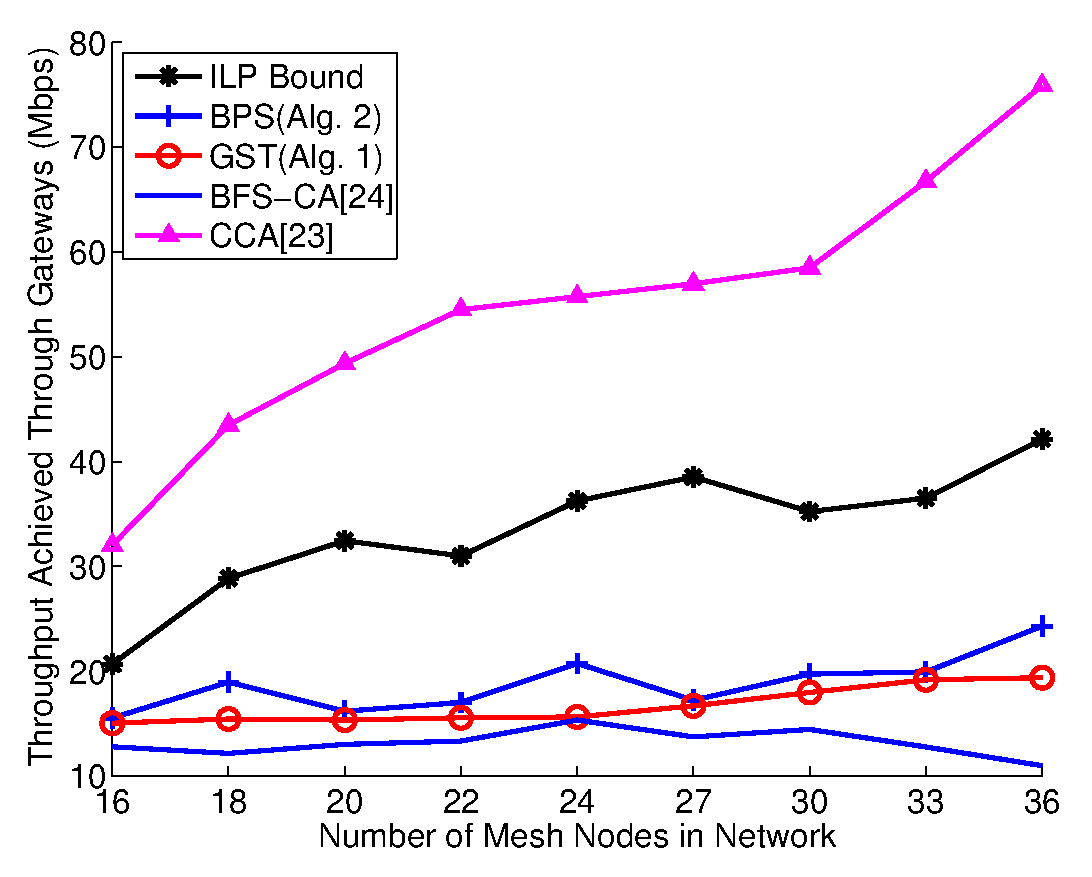
\includegraphics[width=1.6in]{figures/varysize}}
\subfigure[Varying Load, 49-Nodes Regular Grid]{
\label{fig:maxtpt}
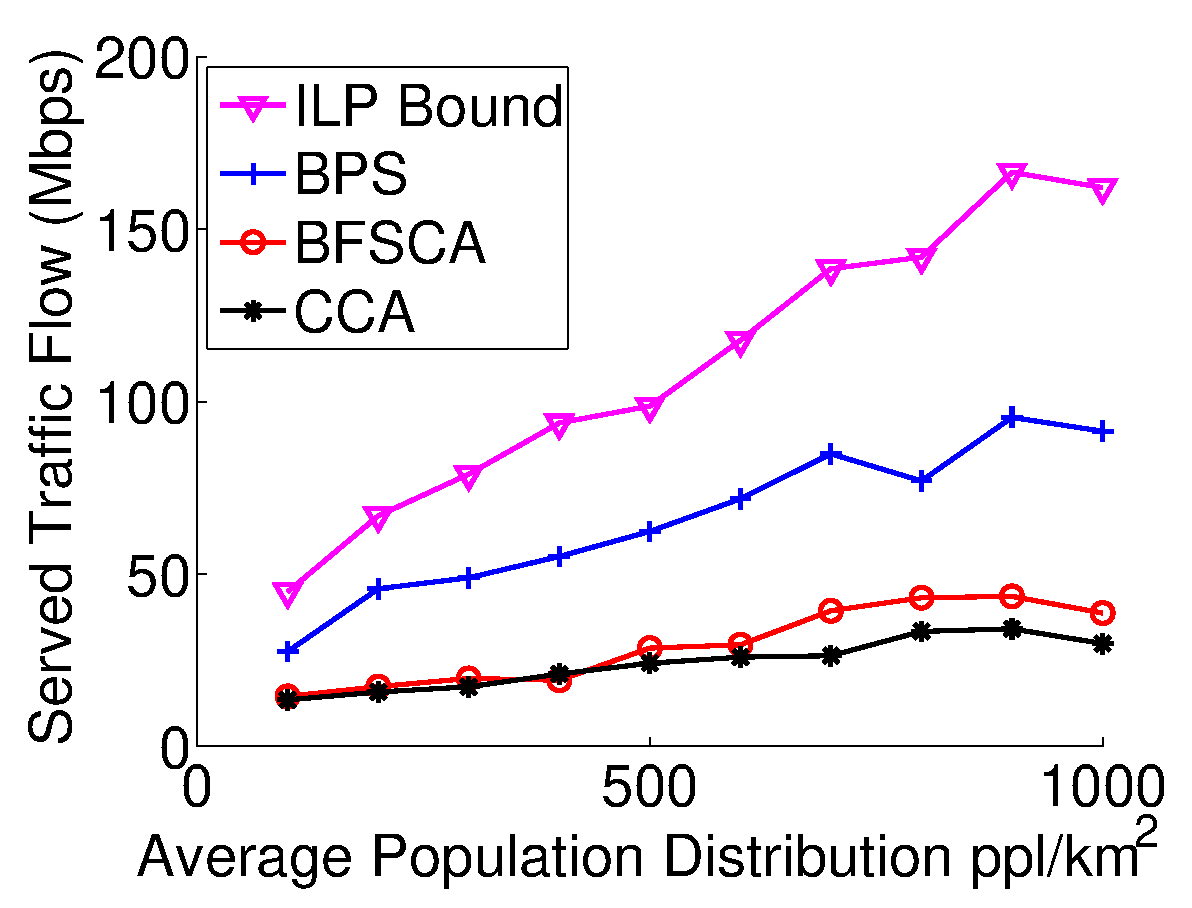
\includegraphics[width=1.6in]{figures/maxtpt.eps}}
\hfill
\caption{Performance in terms of served traffic flow for various offered loads, network sizes, and configurations of WiFi or white space (WS) channels.}
\label{fig:all3figs}
\vspace{-0.1in}
\end{figure}
%\end{figure*}

In Fig.~\ref{fig:varysize}, we observe as the network size increase, the performance
gap among BPS and CCA/BFS-CA goes up. When the network size which represent the size 
of target area, the multiband wireless network has similar communication and interference 
performance with the multi-channel wireless network since all the nodes are located in a 
limited space where could be communicated/interfered by all the bands. As network size 
increase, the connection/interference variation among multiple bands makes the performance 
of multi-channel algorithms stay in low level. The LP Bound shows what could be expected, 
that an increasing number of gateways/mesh nodes produce an increase in total traffic 
arrived gateways. However, we observe that CCA, BFS-CA algorithms are not able to achieve 
such behavior for various reasons. CCA fails to employ the communication range variation 
and find the most efficient hop connections which increase the average hop count. BFS-CA 
optimizes the first connection hop from the gateway, but fails to deal the whole path 
from the gateway to destination node. Conversely, BPS alleviates the strain on these 
first-hop, bottleneck links, achieving average 76\% of the ILP Bound. The gap of BPS 
to the ILP is part from that the BPS only considers static one path to a gateway node for 
each mesh node, whereas the LP allows multiple paths to the gateways. For BPS and other 
heuristic algorithms the dynamic assignment could be implemented through updating the 
assignment in a short term.

\begin{table*}
\centering % centering table 
\begin{tabular}{|c|c|c|c|c|c|c|c|c|c|c|c|} % creating 12 columns 
\hline %\hline % inserting double-line 
%Bands     & \multicolumn{3}{c|}{Dallas} & \multicolumn{3}{c|}{Weatherford} & \multicolumn{3}{c|}{Millsap} \\% [0.5ex]
%\hline % inserts single-line 
% Entering 1st row 
 \multirow{2}{*}{Frequency Bands} & \multicolumn{9}{|c|}{Population Distribution $ppl/km^2$} \\
\cline{2-10}
		& 1500 & 1000 & 500 & 300 &  200 & 150 & 100 & 20 & 10 \\ % [0.5ex]
\hline % inserts single-line 
450 MHz &24.37	&25.83  &23.77	&6.05 &12.50  &14.03 & 7.00 & 0.07 & 0.02 \\      
\hline % inserts single-line                                                                                                       
800 MHz &4.40 	&16.49  &4.77	&5.22&5.07 &4.43  & 3.87 & 4.20 & 3.60 \\      
\hline % inserts single-line                                                                                                      
2.4 GHz &15.87 	&34.95  &2.60	&2.03&2.03 &2.77  & 2.07 & 1.60 & 0.80 \\      
\hline % inserts single-line                                                                                                     
5.2 GHz &19.70	&35.46  &1.53	&1.93&1.93 &1.33  & 1.27 & 2.07 & 2.10 \\      
\hline % inserts single-line 
\end{tabular}    
\caption{Activity Level under Population Distribution} % title name of the table 
\label{tab:activitymeasurement}    
\vspace{-0.3in}
\end{table*}    

% Simulation set up
Next, we consider a different form of scalability in our analysis.  Namely,
we increase the average population distribution from 100 to 1,000 per km$^2$, while
maintaining a 49-node regular grid topology. In the simulation set up, we map the
channel capacity to the closest population measurement results. If there are 
measurements has the same distance to the current set up, the lower population 
measurement will be chosen, for instance, we map $400 ppl/km^2$ to $300 ppl/km^2$ 
measurements as shown in Table.~\ref{tab:activitymeasurement}. In Fig.~\ref{fig:maxtpt},
it shows that as the population distribution increases, the ILP and BPS diverge greatly 
from the remaining algorithms. Similar to Fig.~\ref{fig:varysize}, the wireless channel 
capacity around a gateway is quickly saturated if the algorithm is not focused on 
preserving that resource. Another factor of the performance is the channel capacity, 
as population increase the measured channel capacity vary in different bands.
As the population reaches 1,000, the traffic arrived gateways decrease due to the 
channel capacity and the saturation of wireless channel capacity around the gateway
nodes. BPS has an average performance of 60\% of the ILP Bound, on average. CCA and BFS-CA
fails to serve more traffic demand through the jointly WiFi and white space wireless
network. 

\begin{table*}
\centering % centering table 
\begin{tabular}{|l|c|c|c|c|c|c|c|c|c|c|c|} % creating 12 columns 
\hline %\hline % inserting double-line 
Bands/     & WiFi    & WS      & WS \& & WS \& &  WS \& & WS \& & WS \&      &  WS \&      & Multi-WS \& & Multi-WS \& & Multi-WS \& \\% [0.5ex]
Algorithms & Only    & Only    & WiFi  & WiFi  &  WiFi  & WiFi  & Multi-WiFi &  Multi-WiFi & WiFi        & WiFi        & Multi-WiFi  \\
\hline % inserts single-line 
% Entering 1st row 
WS (MHz)   &                                                        & 450,800 & 450 &  800  &  450   & 800               & 450    & 800      & 450,800     & 450,800     & 450,800     \\
\hline
WiFi (GHz) & 2.4, 5 &                                                             & 2.4 &  2.4  &  5   & 5               & 2.4, 5& 2.4, 5        & 2.4             & 5         & 2.4, 5     \\ % [0.5ex]
\hline
\hline % inserts single-line 
CCA~\cite{draves2004routing}                & 22.4   &  13.4  & 13.2    &12.5    & 16.9       & 23.2   &  24.1  &   30.6&  25.2  &       23.9       &   30.4          \\      
\hline % inserts single-line                                                                                                       
BFS-CA~\cite{ramachandran2006interference}  & 26.3   &  15.8  & 14.9    & 19.4   & 22.7       & 28.4   &  38.9  &   33.7&  30.1  &       27.4       &       36.6      \\      
%\hline % inserts single-line                                                                                                      
%GST (Alg. 1)                                                            & 11.6  &   6.6 & 9.3    &   15.1&   15.8        &  14.4  &   16.6   &    14.1  &   18.8            &  15.0           &    25.1         \\      
\hline % inserts single-line                                                                                                     
BPS (Alg. 1)                                & 41.2   & 34.1   &  38.2  & 40.0    & 35.4       & 42.8   & 58.4   &  64.9 &  54.4  &       51.9       &       63.1      \\      
\hline % inserts single-line 
\end{tabular}    
\caption{Throughput achieved through Gateway nodes (Mbps) for various combinations of WiFi and Average Population Distribution = 500 $ppl/km^2$, Network Size = 49 mesh nodes).} % title name of the table 
% NEWClaim fix
\label{tab:2channelcombination}    
\vspace{-0.4in}
\end{table*}    


WhiteMesh networks could be deployed across a vast array of environments, from
rural to urban areas. Each of these areas will have varying amounts of user
demand traffic in proportion to the population densities.  However, 
since a greater number of TV stations exist in urban areas, the available 
white space bands are often inversely related to the population density due to 
the FCC rules~\cite{fccwhitespace}. Also the available channel capacity is 
related to the existing signal activities in the area. To capture these varying
degrees of demand and white space availability we consider three likely scenarios
and one final scenario for comparison purposes: {\it (i)} two WiFi bands (2.4 and
5.8 GHz) channels with two white space channels (450 and 800 MHz), {\it (ii)} 
three channels in two WiFi bands (2.4 and 5.8 GHz) with one white space channel 
(450 MHz), {\it (iii)} Four channels in two WiFi bands (2.4 and 5.8 GHz) without 
any white space channels, and {\it (iv)} four channels in two white space bands 
(450 and 800 MHz) with no WiFi bands (for comparison).

Table~\ref{tab:2channelcombination} describes the achieved traffic arrived gateways 
for various combinations of WiFi and white space bands with a maximum offered load 
of 5 Mbps from 500 $ppl/km^2$ in a regular 49-node grid. We consider the performance 
of BPS in the four aforementioned scenarios of varying white space availability. A 
regular, 49-nodes grid is again used. In the simulation, we keep 4 channels for each
method, such as in the combination of 2.4 GHz and 5 GHz, we put 2 channels in both 
bands. In the triple bands combinations, we set each band has a channel, and put the 
other channel in the highest frequency band. (In 2.4 GHz, 5GHz, 800 MHz combination, 
we put the extra channel other than the 3 channel each band in 5 GHz). 
% Justification
Immediately, we observe that the WiFi-only scenario has greater traffic arrived 
gateways than the white-space-only scenario. This is due to the lack of spatial 
reuse achieved by white spaces. White space has larger communication to shorten 
the hop counts as well as has larger interference reducing the spatial reuse. 
Another reason is that the available channel capacity of 500 $ppl/km^2$ in white 
space bands are worse than WiFi bands. This two reasons make the white space only 
has worse performance no matter what channel assignment methods are applied.
Interestingly, however, the joint use of both white space and WiFi bands has 
significant gains over the single type of band scenarios with the same number of 
channels (40\% greater than WiFi and 56\% over white space, on average). 

In 500 $ppl/km^2$ scenario, 5 GHz channel is cleaner than 450 MHz which makes 
the combination of 2 channels in 5 GHz, 1 channel in 2.4 GHz and 800 MHz has 
better performance than WiFi(2)+WS(2) in some cases.  Obviously, in Table
~\ref{tab:2channelcombination} that with the same number of available bands (2), 
when the combination has similar propagation characters, such as one in WiFi band, 
one in white space band, the combination has clean channels have better performance. 
With similar channel capacity, lower frequency offers more option for connection 
path could output a better channel assignment. If we have one channel in a white 
space band and one channel in a WiFi band, then we could use the advantage of both 
WiFi for spatial reuse and white spaces to reduce the hop count. 



\subsubsection{Effect of Channel Occupancy}

% FIXME include 3 d figure
In Fig.~\ref{fig:actspac}, we show the impacts of channel occupancy through 
the activity level and spacing variation on wireless white space mesh network. 
The activity level defined in~\ref{eq:intercap} represent the available channel
capacity. The spacing gap is related to the population distribution according to 
the hexagon deployment for access tier network deployment, the more population
distribution, the smaller spacing gap between mesh nodes. In the simulation, we 
assume all the bands have the same activity level and use the 49-nodes regular 
grid with normalized multiple spacing distance gap from 0.2 to 2.1. From the 3-D 
figure, we could see as the activity level increase, the traffic arrived gateways 
decrease due to the deduction of available channel capacity. In the spacing dimension, 
when the nodes have small spacing gap, all the bands could not be applied for 
spacial reuse, the traffic arrived gateways is small. But as the spacing gap 
increase, the spacial reusing is available for high frequency bands, the traffic 
arrived gateways increase. Then, as the spacing gap increase over the high 
frequency communication range, the number of usable channels start to decrease 
according to protocol model, the traffic arrived gateways decrease in the figure.

We further investigate the spacing gap variation under in-field scenario.
The in-field measurement mapping is listed in Table.~\ref{tab:activitymeasurement}. 
We keep the white mesh network as 49-nodes regular grid, assume each mesh 
node has 4 radios in each band. As clarified, a larger spacing gap between mesh 
nodes means less population. We map the largest population distribution in Table
~\ref{tab:activitymeasurement} to represent the spacing as normalized distance 0.2,
and the least population distribution as normalized distance 1.7. 
In a regular grid the spacing distance $D_s$, population distribution $P_d$ and 
mesh node capacity $M_c$ should obey $P_d \cdot \frac{D_s}{2} ^2 \propto M_c$. 
The 9 measured data sets are mapped to generate the matrix sets. Then according 
the data in the matrix we interpolate activity level for each normalized distance 
from 0.2 to 1.7 with gap 0.1. These data sets are put into the heuristic algorithms 
and the results are shown in Fig.~\ref{fig:measurespacing}.

\begin{figure}[t]
\centering
\subfigure[Uniform Activity Level VS. Space Distance]{
\label{fig:actspac}
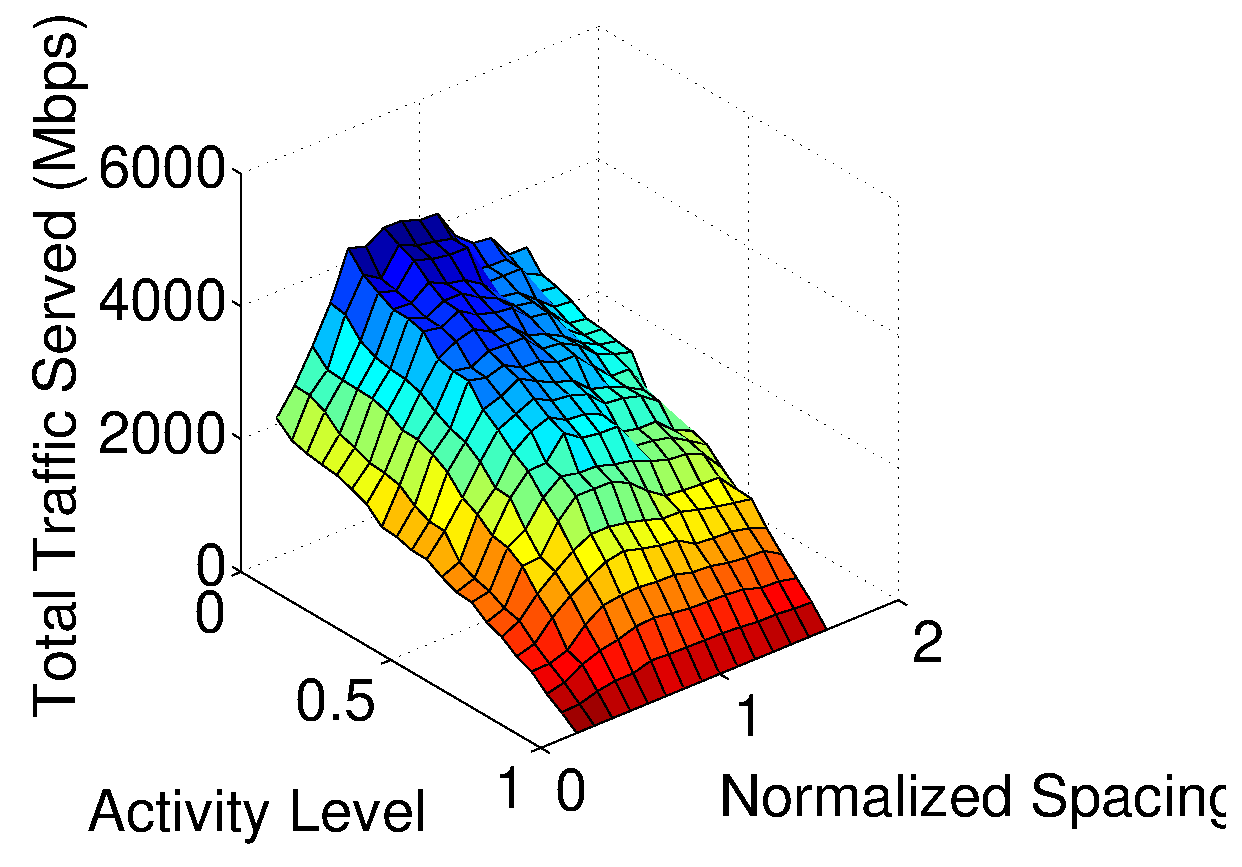
\includegraphics[width=1.6in]{figures/actspac3d}}
\subfigure[Traffic arrived Gateways with Activity Level \& Spacing ]{
\label{fig:measurespacing}
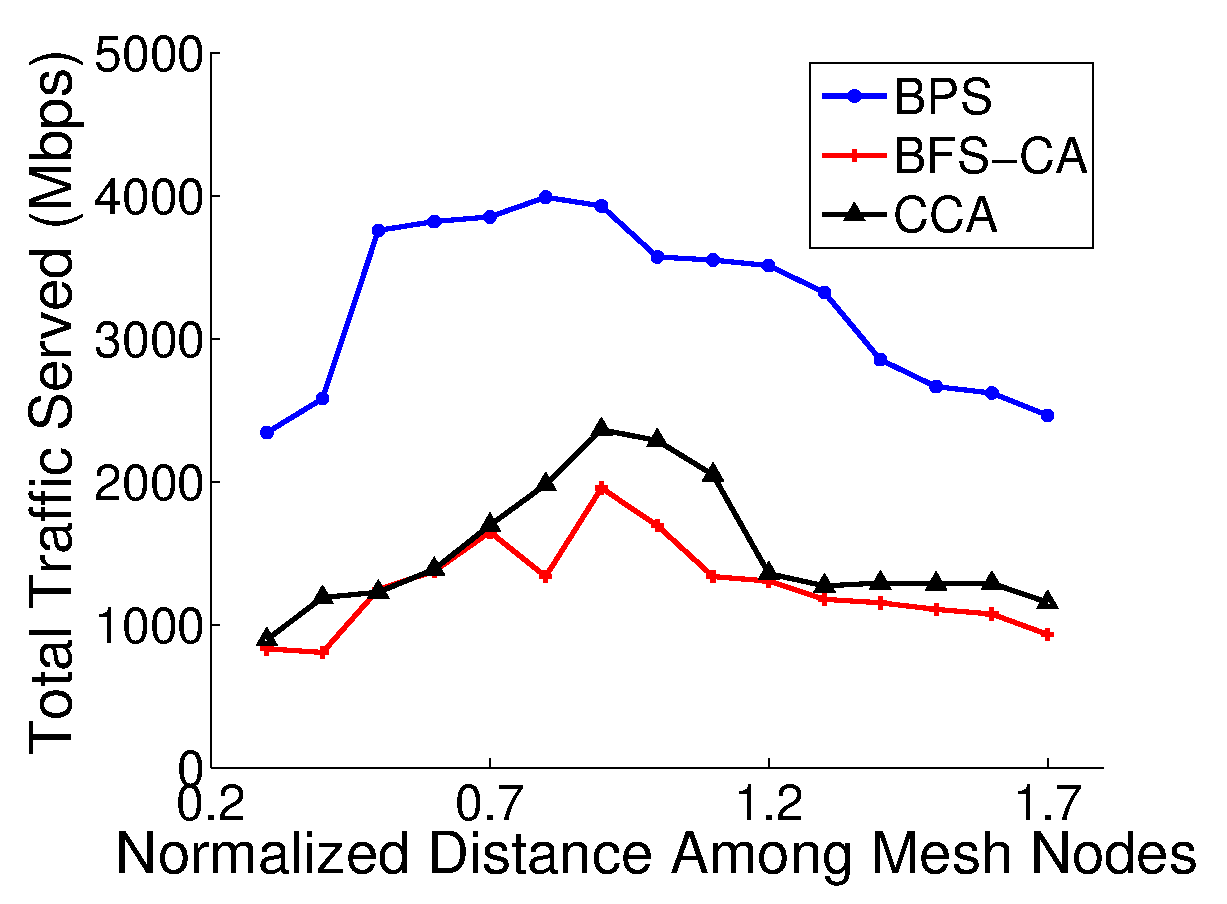
\includegraphics[width=1.6in]{figures/act_spacing}}
\hfill
\caption{}
\label{fig:all3figs}
\vspace{-0.1in}
\end{figure}

In Fig.~\ref{fig:measurespacing}, as the space gap increase, the multiband network 
has better performance through spacial reuse matching the simulation analysis shown 
in Fig.~\ref{fig:actspac}. As the distance increase up to normalized distance 1, one of 
the channel in 5 GHz could not be applied in the network since the distance is larger 
than its communication range under the protocol model, that makes the performance 
decrease quickly. Through this investigation, we can conclude that in sparse area
when the number of mesh nodes is small, lower frequency for the back-hual network 
could have better performance. However, in dense area when the mesh nodes are deployed 
closely, have higher frequency for spacial reuse is better than the low frequency 
white space bands.


Through these analysis, a mixed WiFi and white space wireless network could improve the performance 
in the scenarios as follow: 
{\it (i)} Larger network has more mesh nodes, which 
need more capacity from spacial reuse and flexible path to reduce hop count through
more links. 
{\it (ii)} Rural area whose spacing gap among mesh nodes is larger.
Not only for the number of mesh nodes reducing but also for hop count reducing.
However, as we discussed, the flexible paths and the interference among these
links become more critical at different points in the WhiteMesh topology. 
For the sake of completeness, we need cautious selection of frequency bands
in wireless network deployment.


